\documentclass{beamer}
\usepackage{tikz}
\usetikzlibrary{decorations.pathreplacing, arrows.meta}

\begin{document}

\begin{frame}
\centering

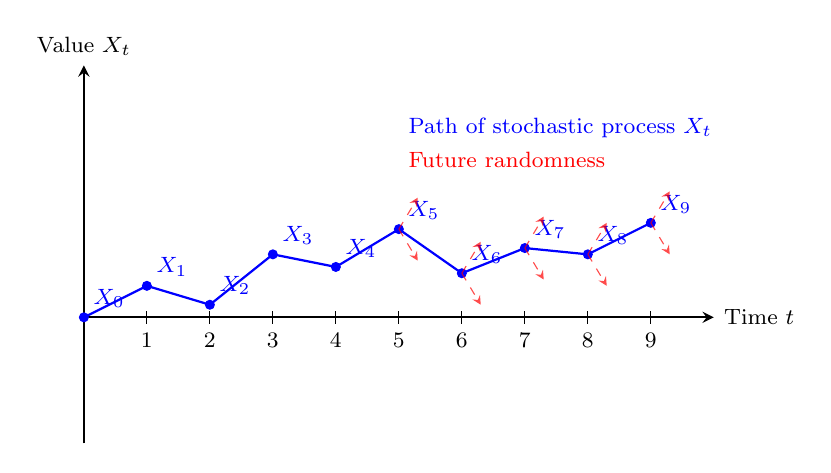
\begin{tikzpicture}[
    >=stealth,
    scale=0.8,
    every node/.style={font=\footnotesize}
]

% Axes
\draw[->, thick] (0,0) -- (10,0) node[right] {Time $t$};
\draw[->, thick] (0,-2) -- (0,4) node[above] {Value $X_t$};

% Time labels
\foreach \x in {1,2,3,4,5,6,7,8,9}
    \draw (\x,0.1) -- (\x,-0.1) node[below] {$\x$};

% Random walk path
\draw[blue, thick] (0,0) 
    -- ++(1,0.5) 
    -- ++(1,-0.3)
    -- ++(1,0.8)
    -- ++(1,-0.2)
    -- ++(1,0.6)
    -- ++(1,-0.7)
    -- ++(1,0.4)
    -- ++(1,-0.1)
    -- ++(1,0.5);

% Points at integer times (states of the process)
\foreach \x/\y in {0/0, 1/0.5, 2/0.2, 3/1.0, 4/0.8, 5/1.4, 6/0.7, 7/1.1, 8/1.0, 9/1.5}
    \filldraw[blue] (\x,\y) circle (2pt) node[above right] {$X_{\x}$};

% Uncertainty at future times
\begin{scope}[dashed, red, opacity=0.7]
    \foreach \x/\y in {5/1.4, 6/0.7, 7/1.1, 8/1.0, 9/1.5} {
        \draw[->] (\x,\y) -- ++(0.3,0.5);
        \draw[->] (\x,\y) -- ++(0.3,-0.5);
    }
\end{scope}

% Labels
\node[blue, right] at (5,3) {Path of stochastic process $X_t$};
\node[red, right] at (5,2.5) {Future randomness};

\end{tikzpicture}

\end{frame}
\begin{frame}

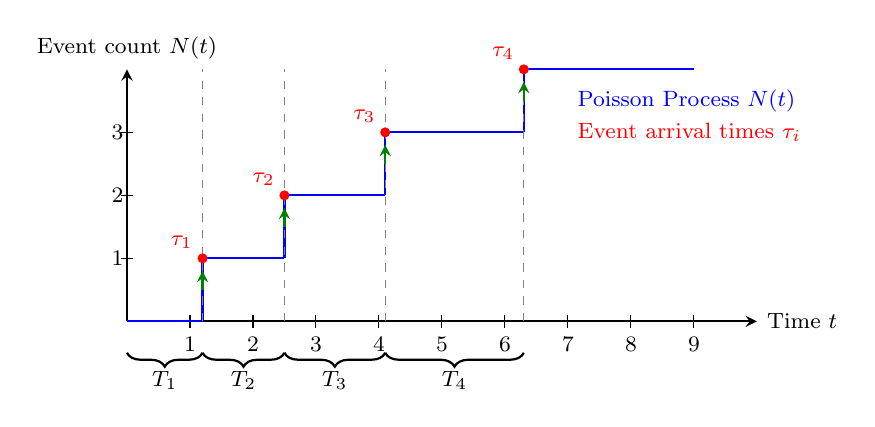
\begin{tikzpicture}[
    >=stealth,
    scale=0.8,
    every node/.style={font=\footnotesize}
]

% Axes
\draw[->, thick] (0,0) -- (10,0) node[right] {Time $t$};
\draw[->, thick] (0,0) -- (0,4) node[above] {Event count $N(t)$ };


% Time labels
\foreach \x in {1,2,...,9}
    \draw (\x,0.1) -- (\x,-0.1) node[below] {$\x$};

% Count labels on y-axis
\foreach \y in {1,2,3}
    \draw (-0.1,\y) -- (0.1,\y) node[left] {$\y$};

% Poisson process jumps (step function)
\draw[blue, thick] (0,0) -- (1.2,0);  % First segment
\draw[blue, thick] (1.2,0) -- (1.2,1);  % First jump
\draw[blue, thick] (1.2,1) -- (2.5,1);  % Second segment
\draw[blue, thick] (2.5,1) -- (2.5,2);  % Second jump
\draw[blue, thick] (2.5,2) -- (4.1,2);  % Third segment
\draw[blue, thick] (4.1,2) -- (4.1,3);  % Third jump
\draw[blue, thick] (4.1,3) -- (6.3,3);  % Fourth segment
\draw[blue, thick] (6.3,3) -- (6.3,4);  % Fourth jump
\draw[blue, thick] (6.3,4) -- (9,4);    % Final segment

% Event arrival times
\foreach \x in {1.2, 2.5, 4.1, 6.3}
    \draw[dashed, gray] (\x,0) -- (\x,4);

% Event markers
\foreach \x/\y in {1.2/1, 2.5/2, 4.1/3, 6.3/4} {
    \filldraw[red] (\x,\y) circle (2pt);
    \node[above left, red] at (\x,\y) {$\tau_{\y}$};
}

% Jumps indicated with arrows
\begin{scope}[green!50!black, thick, ->, >=stealth]
    \draw (1.2,0.5) -- (1.2,0.8);
    \draw (2.5,1.5) -- (2.5,1.8);
    \draw (4.1,2.5) -- (4.1,2.8);
    \draw (6.3,3.5) -- (6.3,3.8);
\end{scope}

% Inter-arrival times
\draw[decorate, decoration={brace, amplitude=5pt, mirror}, thick] (0,-0.5) -- node[below, yshift=-3pt] {$T_1$} (1.2,-0.5);
\draw[decorate, decoration={brace, amplitude=5pt, mirror}, thick] (1.2,-0.5) -- node[below, yshift=-3pt] {$T_2$} (2.5,-0.5);
\draw[decorate, decoration={brace, amplitude=5pt, mirror}, thick] (2.5,-0.5) -- node[below, yshift=-3pt] {$T_3$} (4.1,-0.5);
\draw[decorate, decoration={brace, amplitude=5pt, mirror}, thick] (4.1,-0.5) -- node[below, yshift=-3pt] {$T_4$} (6.3,-0.5);

% Labels
\node[blue, right] at (7,3.5) {Poisson Process $N(t)$};
\node[red, right] at (7,3) {Event arrival times $\tau_i$};

\end{tikzpicture}

\end{frame}

\begin{frame}
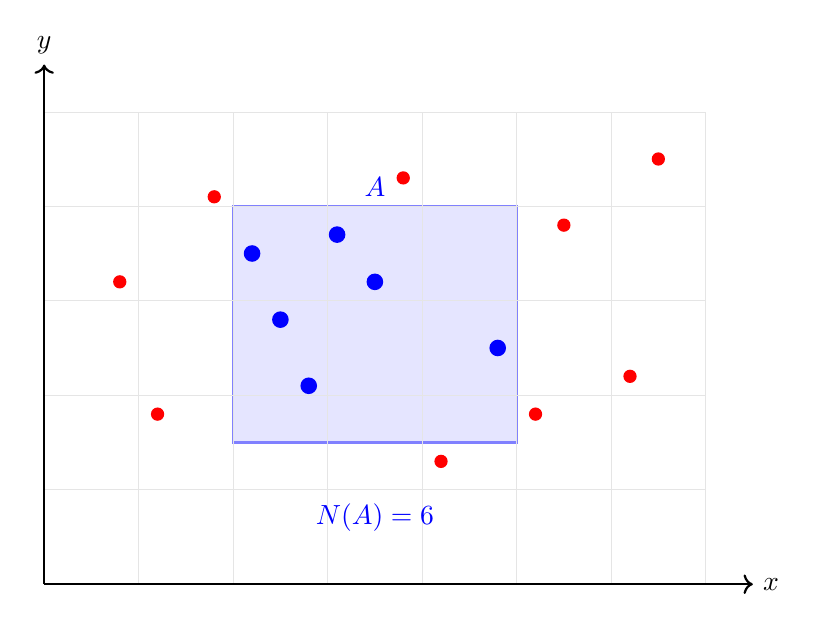
\begin{tikzpicture}[scale=1.2]

% Define the region A
\filldraw[fill=blue!10, draw=blue!50, thick] (2,1.5) rectangle (5,4);
\node[blue] at (3.5,4.2) {$A$};

% Draw a grid for spatial reference
\draw[gray!20, very thin] (0,0) grid (7,5);

% Axes
\draw[->, thick] (0,0) -- (7.5,0) node[right] {$x$};
\draw[->, thick] (0,0) -- (0,5.5) node[above] {$y$};

% Random points scattered in space
\foreach \x/\y in {1.2/1.8, 2.8/2.1, 3.5/3.2, 1.8/4.1, 4.2/1.3, 
                   3.1/3.7, 2.5/2.8, 4.8/2.5, 5.5/3.8, 6.2/2.2,
                   0.8/3.2, 3.8/4.3, 6.5/4.5, 5.2/1.8, 2.2/3.5} {
    \fill[red] (\x,\y) circle (2pt);
}

% Highlight points inside A
\foreach \x/\y in {2.8/2.1, 3.5/3.2, 3.1/3.7, 2.5/2.8, 2.2/3.5, 4.8/2.5} {
    \fill[blue] (\x,\y) circle (2.5pt);
}

% Count label
\node[blue] at (3.5,0.7) {$N(A) = 6$};

\end{tikzpicture}
\end{frame}

\begin{frame}
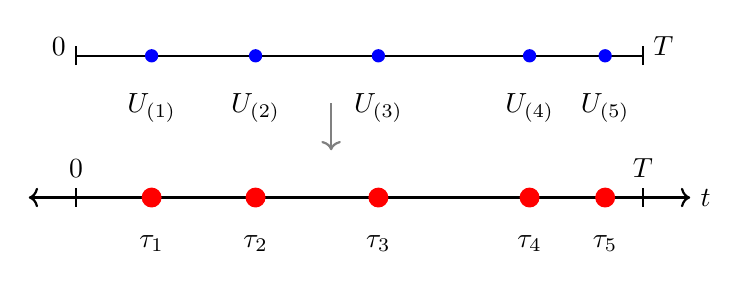
\begin{tikzpicture}[scale=1.2]

% Main timeline
\draw[<->, thick] (-0.5,0) -- (6.5,0) node[right] {$t$};
\draw[thick] (0,-0.1) -- (0,0.1) node[above] {$0$};
\draw[thick] (6,-0.1) -- (6,0.1) node[above] {$T$};

% Poisson points on timeline
\foreach \x in {0.8, 1.9, 3.2, 4.8, 5.6} {
    \fill[red] (\x,0) circle (3pt);
}

% Label points as order statistics
\node[below] at (0.8,-0.3) {$\tau_{1}$};
\node[below] at (1.9,-0.3) {$\tau_{2}$};
\node[below] at (3.2,-0.3) {$\tau_{3}$};
\node[below] at (4.8,-0.3) {$\tau_{4}$};
\node[below] at (5.6,-0.3) {$\tau_{5}$};

\node[below] at (0.8,1.2) {$U_{(1)}$};
\node[below] at (1.9,1.2) {$U_{(2)}$};
\node[below] at (3.2,1.2) {$U_{(3)}$};
\node[below] at (4.8,1.2) {$U_{(4)}$};
\node[below] at (5.6,1.2) {$U_{(5)}$};

% Uniform distribution bar above
\draw[thick] (0,1.5) -- (6,1.5);
\draw[thick] (0,1.4) -- (0,1.6) node[left] {$0$};
\draw[thick] (6,1.4) -- (6,1.6) node[right] {$T$};

% Uniform random points
\foreach \x in {0.8, 1.9, 3.2, 4.8, 5.6} {
    \fill[blue] (\x,1.5) circle (2pt);
}

% Sort arrow
\draw[->, thick, gray] (2.7,1) -- node[right] {} (2.7,0.5);

\end{tikzpicture}\end{frame}

\begin{frame}
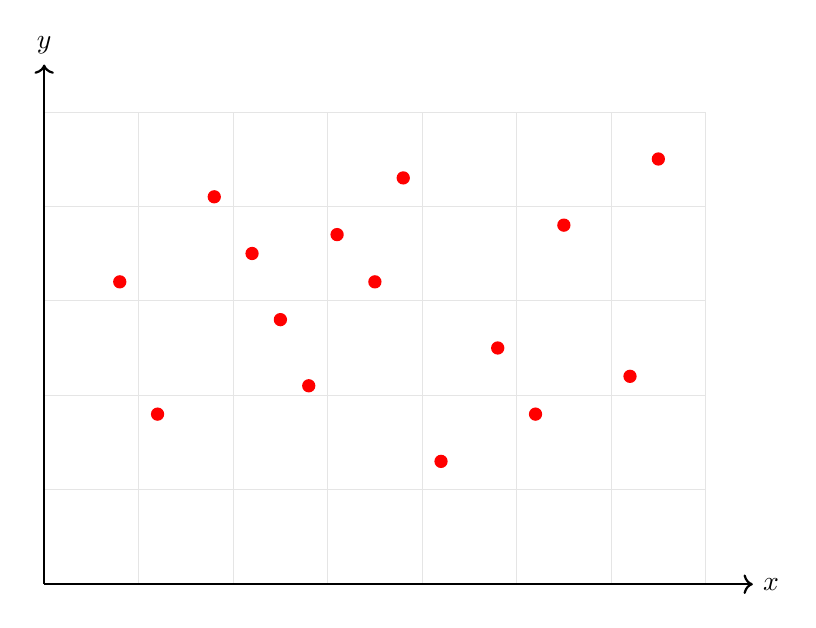
\begin{tikzpicture}[scale=1.2]

% Draw a grid for spatial reference
\draw[gray!20, very thin] (0,0) grid (7,5);

% Axes
\draw[->, thick] (0,0) -- (7.5,0) node[right] {$x$};
\draw[->, thick] (0,0) -- (0,5.5) node[above] {$y$};

% Random points scattered in space
\foreach \x/\y in {1.2/1.8, 2.8/2.1, 3.5/3.2, 1.8/4.1, 4.2/1.3, 
                   3.1/3.7, 2.5/2.8, 4.8/2.5, 5.5/3.8, 6.2/2.2,
                   0.8/3.2, 3.8/4.3, 6.5/4.5, 5.2/1.8, 2.2/3.5} {
    \fill[red] (\x,\y) circle (2pt);
}

\end{tikzpicture}
\end{frame}


\end{document}
